\newlength{\tmpxshift}
\newlength{\tmpyshift}
\newlength{\tmpheight}

\begin{scope}[yshift=\zinepanelheight]
% If you feel a need to cover up the yellow circle in the demo...
%   \fill[color=white] (0.1,-0.1) rectangle (\pzptmpPanelWidth - .2, -1 * \zinepanelheight + .2);

   \newlength{\tmpxshift}
   \pgfmathsetlength{\tmpxshift}{\gxshiftfrac * \pzptmpPanelWidth}

   \newlength{\tmpyshift}
   \pgfmathsetlength{\tmpyshift}{\gyshiftfrac * \zinepanelheight}

   \newlength{\tmpheight}
   \pgfmathsetlength{\tmpheight}{\pzptmpGraphicHeight * \gscale}
   \node[transform shape, xshift=\gxshiftfrac * \pzptmpPanelWidth, yshift=\tmpyshift]
     {\includegraphics[page=9, height=\tmpheight, keepaspectratio]{CarletonEtAl2026.pdf}};
   
\end{scope}
\let\tmpxshift\relax
\let\tmpyshift\relax
\let\tmpheight\relax
